\chapter{Theory}
\label{stheory}
%\subsection{Introduction to Mixing Phenomenology}
\textit{The Standard Model is without question the most powerful and tested theory of particle physics. It describes and predicts many phenomena very well even though as discussed in the previous chapter it fails to address certain known issues. In this chapter, the theoretical basis of the Standard Model is first laid out which is then followed by the experimental and theoretical considerations of fully leptonic decays. The introduction in this chapter is based on Ref\cite{Griffiths:111880},\cite{Novaes:1999yn} and \cite{Pich:2012sx}.}



\section{Review of the Standard Model}
The \gls{SM} of particle physics is currently the most accurate model describing the buildings blocks of matter, particles, and their interactions via forces. In particular the \gls{SM} describes all the fundamental forces but gravity. It is a quantum field theory (\gls{QFT}) whereby the dynamics of the system is captured by the most general renormalisable Lagrangian density that is invariant under gauge symmetry. \gls{QFT} considers particles to be excited states of an underlying field, also known as quanta. In the \gls{SM}, particles and forces are the results of interactions between scalar, vector and spinor fields. In general there are two sets of particles. The first set are force-carrying particles also known as bosons, which have integer spin and are quanta of the scalar and vector fields. More specifically, there is the Higgs boson, the only elementary scalar boson in the \gls{SM}, and vector bosons: gluons, $W^{\pm}$, Z and $\gamma$. Secondly, there are the non-force carrying particles, which are fermions, quanta of spinor fields. Unlike bosons they carry half-integer spin. These can be further classified into two elementary families of particles: quarks, which cannot be observed alone and leptons which can be detected on their own. Out of all of these fundamental particles, those that have mass acquire it by the Higgs mechanism.

%Quarks are affected by all three fundamental forces. They come in six different \textit{flavours} and they carry fractional charge as seen in~\autoref{nonlin}.

\begin{table}
\centering % used for centering table 
\begin{tabular}{c c c c} % centered columns (4 columns) 
\toprule %inserts double horizontal lines 
Generation & Flavour & Charge & Quark Mass \\ [0.5ex]\hline% inserts table 
%heading 
% inserts single horizontal line 
1st & up  \textit{u}& +2/3 & $2.2\bfrac{+0.6}{-0.4}$ \mev \\ % inserting body of the table 
1st & down \textit{d}& -1/3 & $4.7\bfrac{+0.5}{-0.4}$ \mev \\[1ex]
2nd & charm \textit{c}& +2/3 & $1.28\pm0.03$\gev\\
2nd & strange \textit{s}& -1/3 &  $96\bfrac{+8}{-4}$ \mev\\[1ex]
3rd & top \textit{t}& +2/3 &  $173.1\pm0.6$ \gev \\
3rd & bottom \textit{b}& -1/3 & $4.18\bfrac{+0.4}{-0.3}\gev$ \\ [1ex] % [1ex] adds vertical space 
\bottomrule %inserts single line 
\end{tabular}
\caption{Quarks and their properties such as flavour, charge and mass. Flavour is a property which distinguishes different species of quarks. Another property is the mass of the quark. The masses are taken from \cite{Patrignani:2016xqp}.}
\label{nonlin} % is used to refer this table in the text 
\end{table}

%Sallyconstituent mass - binding force



Quarks are affected by all three fundamental forces. They come in six different \textit{flavours} and they carry fractional charge as seen in~\autoref{nonlin}. 

There are also 12 leptons in total. Unlike quarks, they are not affected by the strong force but also come along in three generations with increasing mass: electrons, muons and taus. They all have their antiparticles and corresponding neutrinos. Much of this thesis is dedicated to the study of the muons or antimuons and their neutrinos. 


In the rest of the chapter, the \gls{SM} formulation is introduced starting with the principle of local gauge invariance explained in~\autoref{build}. The strong and electroweak sectors are described in ~\autoref{qcd} and~\autoref{weak} and the necessary process of mass generation in the \gls{SM}, the Higgs mechanism, is covered in~\autoref{higgs}. The effect of the Higgs mechanism on the electroweak sector is then described in~\autoref{mass} resulting in the quark mixing matrix detailed in~\autoref{ckm}. Following sections then discuss the theoretical and experimental status of fully leptonic decays, which are sensitive to elements of the quark mixing matrix. Finally a discussion about the decay model used for the search of \Bmumumu is covered in~\autoref{mydecay}.  

\section{The Principle of Standard Model Building}
\label{build}
In more mathematical terminology, the \gls{SM} is a theory that respects SU(3)$\otimes$SU(2)$\otimes$U(1) symmetries. In this section, the form of the Lagrangian density of the \gls{SM} is motivated. Throughout it is assumed that $\hbar=1$, $c=1$. The Dirac Lagrangian for a spin-$\frac{1}{2}$ non-interacting or free field $\psi$ (spinor field) for a particle with mass $m$ can be written as 
\begin{equation}
\mathcal{L} = i\overline{\psi}\gamma^{\mu}\partial_{\mu}\psi - m\overline{\psi}\psi,
\label{eq:lag_first}
\end{equation}

\noindent where $\gamma^{\mu}$ are $4\times 4$ Dirac matrices and $\mu\in\{0,1,2,3\}$. By using the Euler-Lagrange equation from the relativistic theory

\begin{equation}
	\partial_{\mu}\Big(\frac{\partial{\mathcal{L}}}{\partial(\partial_{\mu}\psi_{i})} \Big) =\frac{\partial \mathcal{L}}{\partial\psi_{i}}
\label{eq:lag_first}
\end{equation}
for $\overline\psi$ in~\autoref{eq:lag_first} the equation 

\begin{equation}
 i\gamma^{\mu}\partial_{\mu}\psi - m\psi = 0
\label{eq:lag_first2}
\end{equation}
can be retrieved. This is the Dirac equation of motion.

The Dirac Lagrangian in~\autoref{eq:lag_first} stays the same under a global phase transformation: $\psi \rightarrow e^{i\phi}\psi$ and $\overline\psi \rightarrow e^{-i\phi}\overline\psi$. However, under a local phase transformation, where $\phi$ is a function of $x^{\mu}$, this is not the case any more. In this case
\begin{equation}
\mathcal{L} \rightarrow \mathcal{L}- (\partial_{\mu}\phi) \overline{\psi}\gamma^{\mu}\psi.
\label{eq:notinv}
\end{equation}

By requiring local gauge invariance for the Lagrangian, it is necessary to add a term to counteract the left-over term in~\autoref{eq:notinv}. Let $\lambda=-\frac{\phi(x)}{q}$ and let $A_{\mu}$ be some new (vector) field which transforms as $A_{\mu} \rightarrow A_{\mu} + \partial_{\mu}\lambda$, then the following Lagrangian

\begin{equation}
	\mathcal{L} = i\overline{\psi}\gamma^{\mu}\partial_{\mu}\psi - m\overline{\psi}\psi - q\overline{\psi}\gamma^{\mu}\psi A_{\mu}
\label{eq:lag_sec}
\end{equation}
stays invariant under a local phase transformation. That is good, however, there is a penalty for introducing a new vector field $A_{\mu}$ which interacts with the spinor field $\psi$ as can be seen in the last part of~\autoref{eq:lag_sec}. It is now necessary to also introduce a non-interacting term for $A_{\mu}$.

The Lagrangian for the non-interacting vector field for a particle with mass $m_{A}$ and field strength $F^{\mu\nu}=\partial^{u}A^{\nu} - \partial^{\nu}A^{u}$ is
\begin{equation}
\mathcal{L}= -\frac{1}{16\pi} F^{\mu\nu}F_{\mu\nu} + \frac{1}{8\pi}m_{A}^{2}A^{\mu}A_{\mu}.
\end{equation}
In order not to spoil the local gauge invariance, it is required that $m_{A}=0$. Hence the full Dirac Lagrangian with local phase invariance introduces a massless vector field $A^{\mu}$ and is of the form

\begin{equation}
	\mathcal{L} = i\overline{\psi}\gamma^{\mu}\partial_{\mu}\psi - m\overline{\psi}\psi - q\overline{\psi}\gamma^{\mu}\psi A_{\mu} -\frac{1}{16\pi} F^{\mu\nu}F_{\mu\nu},
\label{eq:lag_thir}
\end{equation}
which can be recognized as the Lagrangian for quantum electrodynamics (\gls{QED}), whereby the electrons and positrons (quanta of spinor field) are interacting with photons (quanta of vector field). In other words, $A_{\mu}$ is the electromagnetic potential and $q=e$, the current density is hence $J^{\mu}=e\overline{\psi}\gamma^{\mu}\psi$. This represents the $U(1)_{EM}$ part of the SM.

Upgrading from global invariance of the non-interacting Lagrangian in~\autoref{eq:lag_first} to local invariance in one step can be achieved by defining the \textit{covariant derivative}
\begin{equation}
	\mathcal{D}_{\mu} = \partial_{\mu}+ iqA_{\mu},
\end{equation}
where the secret ingredient is to transform the partial derivative in the same way as the field itself.% local gauge transformation.

\section{Quantum Chromodynamics}
\label{qcd}
To require gauge invariance under a local transformation is a powerful tool and it is used throughout the \gls{SM} building. In this section the development of a Lagrangian for Quantum chromodynamics (\gls{QCD}) is explained. \gls{QCD} describes strong interactions or nuclear binding forces and makes use of quarks ($q$). They are observed to be bound either in pairs - mesons ($q\bar{q}$) - or triplets - baryons ($qqq$). The interactions between quarks and gluons are described by the $SU(3)_{C}$ gauge group. The conserving charge associated with the strong force is known as color, hence the subscript $C$. It was experimentally established that there are 3 colors and borrowing from color theory used by painters these colors are red, blue and green. The quark carries color and antiquark anticolor making mesons and baryons colorless. There are 8 quanta of strong interactions known under the name gluons.

With these constraints, and by requiring the free Lagrangian to be invariant under local $SU(3)$ transformation similarly to the \gls{QED} case, the \textit{covariant derivative}

\begin{equation}
\mathcal{D}_{\mu} = \partial_{\mu} - ig_{s}\frac{\lambda^{a}}{2}G^{a}_{\mu}
\end{equation}
 that respects $SU(3)$ symmetry is obtained, with $\lambda^{a}$ the Gell-Mann matrices, $a\in\{1..8\}$ (8 possible gluons) and $g_{s}$ the strong coupling constant. The field strength for the gluon field is defined as $G_{a}^{\mu\nu}=\partial^{u}G_{a}^{\nu} - \partial^{\nu}G_{a}^{u} + g_{s}f^{abc}G_{b}^{\mu}G_{c}^{\nu}$, where $f^{abc}$ are so-called structure constants which satisfy the following commutation relation:

\begin{equation}
	\Big[\frac{\lambda^{a}}{2},\frac{\lambda^{b}}{2}\Big] = if^{abc}\frac{\lambda^{c}}{2}.
\end{equation}
As compared to the \gls{QED} field, there is an additional term involving gluon fields themselves, causing cubic and quartic gluon interactions, which were not present before.

Another interesting behaviour of the strong interaction is that the quarks are not observed in isolation. This is due \textit{confinement} which can be understood within the framework of \gls{QFT} theory by observing evolution of the coupling strength $g$ as a function of energy scale, also known as $\beta$ function.
The $\beta$-function for a coupling constant $g$ in the \gls{SM} to the two loop contribution takes the following form:
\begin{equation}
\beta_g = \mu {{d g}\over d \mu} = {1\over16\pi^2} \beta_g^{(1)}
+ {1\over(16\pi^2)^2} \beta_g^{(2)},
\end{equation}
where $\beta_g^{(1)},~ \beta_g^{(2)}$ denote the one-loop and two-loop
contributions respectively, and $\mu$ is the energy scale. For the strong interaction, unlike the electromagnetic and weak interactions, $\beta_g$ is negative. For low energies as $\mu \rightarrow 0$ the coupling is very high and hence quarks cannot be observed on their own, \textit{confinement}. On the other hand as $\mu \rightarrow \infty$, or at high energies, the coupling gets small, particles get decoupled, which is known as \textit{asymptotic freedom}. 

The full Lagrangian density for the strong interaction is

\begin{equation}
	\mathcal{L}_{QCD} = i\overline{\psi}\gamma^{\mu}\mathcal{D}_{\mu}\psi - m\overline{\psi}\psi -\frac{1}{4} G_{a}^{\mu\nu}G^{a}_{\mu\nu} = i\overline{\psi}\gamma^{\mu}\partial_{\mu}\psi - m\overline{\psi}\psi + g_{s}\overline{\psi}\gamma^{\mu}\frac{\lambda^{a}}{2}\psi G^{a}_{\mu} -\frac{1}{4} G_{a}^{\mu\nu}G^{a}_{\mu\nu},
\label{eq:lag_fourth}
\end{equation}
where the interaction between quarks and gluons is encoded in the third term.


\section{Electroweak Unification}
\label{weak}
The idea behind unification of the weak and electromagnetic interactions is very powerful, as it has to accommodate for forces that act with very different strength with force-carrying particles that are both massive ($W^{\pm}$,$Z$) and massless ($\gamma$). Furthermore $W^{\pm}$ bosons only couple to left-handed particles, whereas the $Z^{0}$ boson couple to both left and right-handed particles. 
%Furthermore, electromagnetic vertex factor is purely vectorial($\gamma^{\mu}$) whereas $W^{\pm}$ coupling has both axial and vector components: ($\gamma^{\mu}(1-\gamma^{5})$), where $\gamma^{5}=i\times\gamma^{0}\times\gamma^{1}\times\gamma^{2}\times\gamma^{3}$. This last issue can be solved by absorption of $1-\gamma^{5}$ into a spinor field itself.
%In this way
To aid with the situation, the spinor field can be decomposed into left-handed and right-handed (chiral) spinor components
\begin{equation}
	\psi=\psi_{L}+\psi_{R} = P_{L}\psi + P_{R}\psi,
\end{equation}
where $P_{L} =\frac{1-\gamma^{5}}{2}$ and $P_{R}=\frac{1+\gamma^{5}}{2}$ are known as the projection operators. By calling these operators left-handed and right-handed, there is a misconception that $\psi_{L}$ is a helicity eigenstate, but this is only true given the particle in question is massless. These spinors are known to have chirality - known as left or right-handedness. Helicity is rather the projection of the spin on the direction of the momentum.

The spinor field decomposition has an impact on electromagnetic currents, weak currents as well as the fermion mass terms. Firstly, the fermion mass term mixes both left handed and right handed spinors as 

\begin{equation}
	m\overline{\psi}\psi=m(\overline{\psi_{R}}\psi_{L} + \overline{\psi_{L}}\psi_{R}).
\label{eq:mixingpsi}
\end{equation}	
Secondly the electromagnetic current is not mixing the left and right handed components, since $\overline{\psi}\gamma^{\mu}\psi=\overline{\psi_{R}}\gamma^{\mu}\psi_{R} + \overline{\psi_{L}}\gamma^{\mu}\psi_{L}$. Finally weak charged current only acts on left-handed fermions as $\frac{1}{2}\overline{\psi}\gamma^{\mu}(1-\gamma_{5})\psi = \overline{\psi_{L}}\gamma^{\mu}\gamma_{L}$.   


Another observation is that the charged weak interaction only couples leptons within the three generations. This motivates left-handed isospin doublets where for the first generation of fermions

\begin{equation}
%\begin{split}
Q_{L} = \binom{u_{L}}{d_{L}}, ~L_{L} = \binom{e_{L}}{\nu_{L}},
%\end{split}
	\label{eq:defdou}
\end{equation}
and right-handed isospin singlets for up-type quarks, down-type quarks and charged leptons:

\begin{equation}
	u_{R}=(u_{R},c_{R},t_{R}),~
	d_{R}=(d_{R},s_{R},b_{R}),~
	l_{R}=(e_{R},\mu_{R},\tau_{R}).
	\label{eq:defsin}
\end{equation}
The simplest group with doublet representation is SU(2) and in combination with the electromagnetic interaction forms $SU(2)_{L} \otimes U(1)_{Y}$. The conserving charges are inter-related 

\begin{equation}
Q=I^{3} + \frac{1}{2}Y,
\end{equation}
where $I$ refers to weak isospin, $Y$ refers to weak hypercharge, and $Q$ is electric charge.

Again by assuming gauge invariance under local transformation the \textit{covariant derivative} of $SU(2)_{L}\otimes U(1)_{Y}$ is 

\begin{equation}
	D_{\mu} = \partial_{\mu} + i\frac{g}{2}W_{\mu}^{i} \frac{\sigma^{i}}{2} - i \frac{g'}{2}B_{\mu}. 
\label{eq:covdev}
\end{equation}
Here $\sigma^{i}$ are Pauli matrices, $g,g'$ are the electroweak couplings and $W_{\mu}^{i}$ where $i\in\{1,2,3\}$ and $B_{\mu}$ are the vector fields that should be corresponding to $W^{\pm},Z^{0},\gamma$.
The field strengths are defined as $B^{\mu\nu}=\partial^{u}B^{\nu} - \partial^{\nu}B^{u}$ and $W^{i}_{\mu\nu} = \partial^{\mu}W^{i}_{\nu} - \partial^{\nu}W^{i}_{\mu}+ g\epsilon^{ijk}W_{\mu}^{j}W_{\nu}^{k}$.

The real charged bosons corresponding to $W^{\pm}$ arise as linear combinations of $W^{i}_{\mu}$, for $i\in\{1,2\}$ as
\begin{equation}
\begin{split}
W^{\pm}_{\mu} = \frac{1}{\sqrt{2}}(W^{1}_{\mu}\mp iW^{2}_{\mu}),
\\
W_{\mu} \equiv W^{-}_{\mu},
\\
W^{\dagger}_{\mu} \equiv W^{+}_{\mu}. 
\end{split}
\end{equation} 
The neutral bosons are obtained using $W_{\mu}^{3}$ and $B_{\mu}$ in a similar fashion as


\begin{equation}
	Z_{\mu}=-B_{\mu}sin\theta_{W}+W^{3}_{\mu}cos\theta_{W}
\end{equation}
\begin{equation}
	A_{\mu}= B_{\mu}cos\theta_{W}+W^{3}_{\mu}sin\theta_{W},
\end{equation}
where $\theta_{W}$ angle is known as weak mixing angle and can be determined experimentally from the masses of the $Z$ and $W^{\pm}$ bosons by the relation
$cos\theta_{W} = \frac{M_{W}}{M_{Z}}$. So far, however, there was no consideration of how bosons or fermions for that matter become massive which will be covered in the next section.

The full Lagrangian of the electroweak theory then consists of the kinetic part
\begin{equation}
\mathcal{L}_{kin}=  -\frac{1}{4} B^{\mu\nu}B_{\mu\nu} -\frac{1}{4} W_{i}^{\mu\nu}W^{i}_{\mu\nu}
\end{equation}
where for $W_{i}^{\mu\nu}$, like in \gls{QCD}, there is cubic and quartic self interaction amongst the gauge fields. Then there are interactions between the quark/lepton fields and the gauge bosons where it is conventional to split these into two categories according to the charge of the gauge bosons.
This is what gives rise to charged and neutral currents for the electroweak interactions. So employing the physical gauge boson representation, charged current Lagrangian $\mathcal{L}_{CC}$ and neutral current Lagrangian $\mathcal{L}_{NC}$ for one family of fermions reads as
\begin{equation}
	\mathcal{L}_{CC}= - \frac{g}{2\sqrt{2}}\Big[W_{\mu}^{\dagger}\big[\overline{\nu}\gamma^{\mu}(1-\gamma_{5})l + \overline{u}\gamma^{\mu}(1-\gamma_{5})d\big] + h.c\Big], 
\label{eq:LC}
\end{equation}

\begin{equation}
	\mathcal{L}_{NC}= - g sin\theta_{W}(\overline{l}\gamma^{\mu}l)A_{\mu} - \frac{g}{2cos\theta_{W}}\sum_{\psi=\nu,l} \overline{\psi_{i}}\gamma^{\mu}(g^{i}_{V} - g^{i}_{A}\gamma_{5})\psi_{i}Z_{\mu}
\label{eq:NC}
\end{equation}
where \mybox{\color{red} the famous (V-A) structure of the weak charged current} can be seen. The first part of $\mathcal{L}_{NC}$ can be recognized as electromagnetic interaction realising that $e=gsin\theta_{W}$. 

If the field is considered to be under U(1) charge then it was shown that this gauge field was invariant in the QED case. However under SU(2), only left-handed fields transform and hence for the fermionic mass term, which mixes right-handed and left-handed terms as shown in~\autoref{eq:mixingpsi}, gauge invariance is broken.
%there is a transformation whereby $l_{L}$ is transformed into $\nu_{L}$.
For this very reason and also to give mass to the gauge bosons the Higgs mechanism is introduced.

\section{The Higgs Mechanism}
\label{higgs}
The Higgs mechanism introduce a new scalar field with potential $V$ into the model. Through the process known as spontaneous symmetry breaking, it allows fermions and gauge bosons to have a mass term in their Lagrangians while retaining gauge invariance. Let $\phi$ be a doublet of complex scalar fields where

\begin{equation}
\phi = \binom{\phi^{+}}{\phi^{0}},
\end{equation}
where $\phi^{+} = \frac{\phi_{1} + i{\phi_{2}}}{\sqrt{2}}$ and $\phi^{0} = \frac{\phi_{3} + i{\phi_{4}}}{\sqrt{2}}$ so that $\phi^{\dagger}\phi = \frac{\phi_{1}^{2} + \phi_{2}^{2} + \phi_{3}^{2} + \phi_{4}^{2}}{2}$.  The Lagrangian for this field is then

\begin{equation}
	\mathcal{L}_{Higgs} = (D_{\mu}\phi)^{\dagger}(D^{\mu}\phi) + V = (D_{\mu}\phi)^{\dagger}(D^{\mu}\phi) - \mu^{2}\phi^{\dagger}\phi - \lambda (\phi^{\dagger}\phi)^{2},
\end{equation}
where $D_{\mu}$ is given in~\autoref{eq:covdev}, and $V$ is the famous Mexican hat potential where the x-axis is $\phi_{1}$ and the y-axis is $\phi_{2}$. It is required that $\lambda>0$ in order for it to be a ground state.

By finding the ground state - or the stable minimum - of this potential with $\mu^{2}<0$, one gets infinite number of this minima such that
\begin{equation}
	\phi\phi^{\dagger}=\frac{-\mu^{2}}{2\lambda}=\frac{v^{2}}{2}.
\end{equation}
This is the same as saying that the minimum is independent of direction as it lies on a circle of minima. As the minimum is usually known as vacuum, $v$ is called the vacuum expectation value. By choosing a particular minimum, one fixes the direction, and the symmetry of $SU(2)\otimes U(1)$ is spontaneously broken, meaning that the overall theory is symmetrical but the ground state exhibits asymmetry. By convention, the direction $\phi=\frac{1}{\sqrt{2}}\binom{0}{v}$ is chosen. Detailing both real and imaginary part of the fields, the direction can be translated so that $\phi_{3}=\frac{v}{2}$ $\phi_{1}=\phi_{2}=\phi_{4}=0$. This allows for the generation of three massive bosons $W^{\pm}$ and $Z^{0}$, and the massless $\gamma$ of the electroweak theory. The Higgs boson itself arises as an excited quanta around the minimum 

\begin{equation}
\phi=\frac{1}{\sqrt{2}}\binom{0}{v+H}.
\label{eq:ref}
\end{equation}


\section{Fermion Mass Generation}
\label{mass}
Moreover, introducing an additional scalar doublet into the model fixes the broken gauge symmetry for fermionic mass mentioned in~\autoref{eq:mixingpsi} as it is possible to construct the fermion-scalar interaction Lagrangian that is gauge invariant, usually denoted as the Yukawa Lagrangian $\mathcal{L}_{Y}$. It is made up of the leptonic part and the quark part:

\begin{equation}
	\mathcal{L}_{Y}= \mathcal{L}_{L} + \mathcal{L}_{Q}.
\end{equation}
The leptonic term for one family of leptons using definitions in~\autoref{eq:defdou} and~\autoref{eq:defsin} is
\begin{equation}
	\mathcal{L}_{L}= g_{l}(\overline{L}_{L}\phi l_{R} + \overline{l}_{R} \phi^{\dagger} L_{L}), 
	\label{eq:SSB1}
\end{equation}
With $\phi_{c}=\binom{\phi^{0*}}{\phi^{-}}$, the full three generation quark term is
\begin{equation}
	\mathcal{L}_{Q}= y^{u}_{ij}\overline{Q}^{i}_{L}\phi u^{j}_{R} + {y}^{d}_{ij}\overline{Q}^{i}_{L}\phi_{c} d^{j}_{R} + h.c .,
	\label{eq:SSB2}
\end{equation}
where h.c stands for Hermitian conjugate, $i,j$ are the generations, $y^{q}$ are $3\times3$ matrices defining strengths between generations with each $y^{q}$. After spontaneous symmetry breaking (\autoref{eq:ref}), the leptonic interaction term becomes
\begin{equation}
	\mathcal{L}_{L}= \frac{g_{l}v}{\sqrt{2}}(\overline{l}_{L}l_{R} + \overline{l}_{R}l_{L}) + \frac{g_{l}}{\sqrt{2}}(\overline{l}_{L} l_{R}+\overline{l}_{R} l_{L})H = m_{l}(\overline{l}_{L}l_{R} + \overline{l}_{R}l_{L})(1+\frac{H}{v}),
        \label{eq:SSB3}
\end{equation}
where the mass term is then defined as $m_{l}=\frac{g_{l}v}{\sqrt{2}}$. In a similar way for quarks,


\begin{equation}
	\mathcal{L}_{Q}=\frac{v}{\sqrt{2}}(y^{d}_{ij}\overline{u}^{i}_{L} u^{j}_{R} + {y}_{ij}^{d}\overline{d}^{i}_{L} d^{j}_{R} + h.c)(1+\frac{H}{v}).
	\label{eq:SSB4}
\end{equation}
where the quark masses are grouped into $3\times3$ complex matrices of up-type quark (down-type quark) $M^{u}_{ij}=\frac{v}{\sqrt{2}}y_{ij}^{u}$ ($M^{d}_{ij}=\frac{v}{\sqrt{2}}y_{ij}^{d}$).
In conclusion, before the spontaneous breakdown of the electroweak symmetry, all quarks and leptons were massless. Once the Higgs scalar field acquires a vacuum expectation value implying a broken symmetry, quarks and leptons acquire mass. It is then possible to decompose a complex matrix into two distinguishable unitary and one diagonal matrix. The mass matrices can be diagonalised by unitary transformations $U_{uL}$ and $ U_{dL}$ in the following way:
\begin{equation}
\begin{split}
	\mathcal{M}_{u} = U^{\dagger}_{uL}M^{u}U_{uR} = Diag\{m_{u},m_{c},m_{t}\},
\\
	\mathcal{M}_{d} = U^{\dagger}_{dL}M^{d}U_{dR} = Diag\{m_{d},m_{s},m_{b}\}.
\end{split}
	\label{eq:unit}
\end{equation}

This way of diagonalising mass matrices is the most general case of a weak basis transformation which transforms a system to a different basis without altering the physics. Such a transformation is equivalent to changing quark fields from the basis of flavour eigenstates to that of mass eigenstates.
\mybox{\color{red} Ulrik removed sentense: In particular for $q\in(u,d)$}

\begin{equation}
\begin{split}
q'_{L} \equiv U_{qL} q_{L},
\\
q'_{R} \equiv U_{qR} q_{R}.
\end{split}
\end{equation}

This change into the mass eigenstate basis does not affect most of the Lagrangian. More specifically, there will be no change to the $\mathcal{L}_{NC}$ in~\autoref{eq:NC} when expressed in mass eigenstates (hence at tree-level there are no flavour changing neutral-currents in the \gls{SM}), however, charged current $\mathcal{L}_{CC}$ in~\autoref{eq:LC} is affected. Due to the diagonalisation of the mass matrices, $\mathcal{L}_{CC}$ now includes non diagonal couplings for the current as seen in the $\mathcal{L}_{CC}$ for all three fermion generations:

\begin{equation}
	\mathcal{L}_{CC}= - \frac{g}{2\sqrt{2}}\Big[W^{\dagger}_{\mu}\big[\sum_{l}\overline{\nu}\gamma^{\mu}(1-\gamma_{5})l + \sum_{ij}\overline{u_{i}}\gamma^{\mu}(1-\gamma_{5})V_{ij}d_{j}\big] + h.c\Big], 
\label{eq:LC}
\end{equation}
In this equation there is a new term $V_{ij}=V_{CKM}= U_{uL} U_{dL}^\dag$ which is the Cabibbo-Kobayashi-Maskawa (CKM) mixing matrix. From~\autoref{eq:unit} it follows that $V^{\dagger}_{CKM}V_{CKM}=1$, or that \gls{CKM} mixing matrix is unitary by assuming that only the charged current via $W$ will lead to a transition from the up-quark to down-type quark sector. Therefore the CKM matrix elements provide the probabilities of how a $W^{\pm}$ bosons decay.
 

%\begin{equation}\label{weakcurr}
%J_{\mu L}^-= U_{L}^{\dagger}\gamma_\mu V_{CKM}D_{L},
%\end{equation}




\section{The Quark Mixing Matrix}
\label{ckm}
As mentioned above, from the transformation of the mass matrix using two unitary matrices one obtains the \gls{CKM} matrix which exhibits a strong hierarchy in the size of the matrix elements. From the previous discussion the quark mixing matrix is a $3 \times 3$ complex unitary matrix yielding 18 parameters to start with. Unitarity of the \gls{CKM} matrix implies that matrix elements are orthonormal, reducing the count of free parameters to 9. Further, 5 out of 6 quark phases can be absorbed into the redefinition of the quark field, cutting the number of parameters down to 4 parameters, three quark mixing angles and one CP (charge-parity) violating phase. There are many different parametrisations which are all mathematically equivalent to the \gls{CKM} matrix, but the standard parametrisation of the \gls{CKM} matrix for flavour mixing is

\begin{align}
V_{\rm CKM} &=  \begin{pmatrix}   V_{ud} & V_{us} & V_{ub} \cr
    V_{cd} & V_{cs} & V_{cb} \cr
    V_{td} & V_{ts} & V_{tb} \cr \end{pmatrix} \\
 &= \begin{pmatrix}c_{12}c_{13}& s_{12}c_{13} & s_{13}\exp(-i\delta) \cr
-s_{12}c_{23}-c_{12}s_{23}s_{13}\exp(i\delta) & c_{12}c_{23}- 
s_{12}s_{23}s_{13}\exp(i\delta) & s_{23}c_{13} \cr 
s_{12}s_{23}- c_{12}c_{23}s_{13}\exp(i\delta) & 
-c_{12}s_{23}-s_{12}c_{23}s_{13}\exp(i\delta) & c_{23}c_{13}\end{pmatrix},
\end{align}
where $s_{ij} = \sin(\theta_{ij})$ and $c_{ij} = \cos(\theta_{ij})$, $\theta_{12}$ , $\theta_{23}$, $\theta_{13}$ are Euler angles and $\theta_{12}$ is also known as the Cabibbo angle.

A parametrisation reflecting the hierarchical nature in flavour mixing, which is an expansion in terms of the small parameter $\lambda$, was introduced by Wolfenstein\cite{wolf}. The four Wolfenstein parameters are related to the standard parametrization via the following expressions:
\begin{equation}
\begin{split}
\lambda = s_{12}, \\
\qquad
A\lambda^{2} = s_{23}, \\
\qquad
A\lambda^{3}(\rho - i\eta) = s_{13}exp(-i\delta),\\
\end{split}
\end{equation}

\begin{equation}V_{\rm CKM_{Wolfenstein}} = \begin{pmatrix}\circledb{1-\lambda^2/2} & \circledm{\lambda} & \circledss{}A\lambda^3(\rho-i\eta) \cr
	\circledm{-\lambda} & \circledb{1-\lambda^2/2} & \circleds{A\lambda^2} \\
\circledss{}A\lambda^3(1-\rho-i\eta) & \circleds{-A\lambda^2} & \circledb{1}\end{pmatrix} + {\cal O}\left( \lambda^4 \right). \
\end{equation}

A geometrical interpretation of $CP$ violation is offered by the concept of unitarity triangles. Unitarity of the \gls{CKM} matrix can be summarized by two sets of orthogonality relations:
$\sum_{k} |V_{ik}|^2 = \sum_{i} |V_{ik}|^2 = 1$ for all $i$ generations and $\sum_k V_{ik}V^*_{jk} = 0$ for all $i\neq j$. One of the unitary constraints of the \gls{CKM} matrix explicitly states:
\begin{equation}
  V_{ud}V^*_{ub} + V_{cd}V^*_{cb} + V_{td}V^*_{tb} = 0 \, .
\end{equation}
Dividing this constraint by $V_{cd}V^*_{cb}$ and using the relations 
\begin{equation}
   {\rho} + i {\eta} = \frac{\sqrt{A^{4}\lambda^{4}}(\bar{\rho} + i \bar{\eta})}{\sqrt{1-\lambda^2}[A^{4}\lambda^{4}(\bar{\rho} + i \bar{\eta})]}
\end{equation}
 where $\bar{\rho}$ and $\bar{\eta}$ are defined
\begin{equation}
\bar{\rho} \approx \rho - \frac{\rho\lambda^{2}}{2},
\end{equation}
\begin{equation}
\bar{\eta} \approx \eta - \frac{\eta\lambda^{2}}{2},
\end{equation}
the constraint can be pictorially represented in the $\bar{\rho}$ and $\bar{\eta}$ plane as a triangle shown in~\autoref{fig:unitr}.
\begin{figure}[h]
\centering
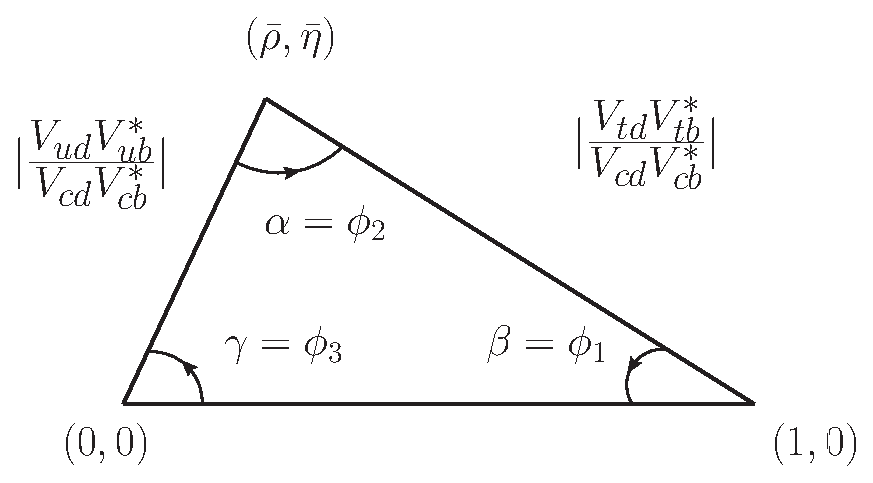
\includegraphics[width=0.5\textwidth]{theory/unitarity.eps}
\caption{Unitarity triangle in a complex plane.}
\label{fig:unitr}
\end{figure}
The area of the triangle is half of the Jarlskog invariant \textit{J}, a quantifier of CP violation, which is defined as $\rm{Im}[V_{ij}V_{kl}V^*_{il}V^*_{kj}]$ \cite{Jarlskog:1985ht}. It is interesting to notice that the \gls{SM} with its parameters may or may not violate CP. Only after measuring \textit{J} it is possible to determine the CP non-conservation. \textit{J} vanishes only if the mixing angle $\theta_{ij} = \{0 , \pi/2\}$; $\delta = \{0 , \pi\}$. So measurements of \textit{J} allows to verify that the \gls{CKM} matrix is complex and hence different mixing for quarks and anti-quarks is obtained.% although \gls{SM} CP violation is not big enough to explain the matter dominated universe.

The \gls{CKM} matrix elements which comprise of magnitudes and phases can be determined in different ways but the most precise option employs a global fit to all available measurements as shown in~\autoref{fig:unifit}. Hence, the most precise measurement of the \gls{CKM} matrix magnitudes to-date \cite{Patrignani:2016xqp} is 
%\begin{equation}|V_{\rm CKM}| = \begin{pmatrix}0.97446 \pm 0.00010 & 0.22452 \pm 0.00044  & \colorboxed{green}{0.00365\pm 0.00012} \cr
%	0.22438 \pm 0.00044 &  0.97359 \bfrac{+0.00010}{-0.00011} & 0.04214\pm 0.00076 \cr
%0.00896 \bfrac{+0.00024}{-0.00023} & 0.04133 \pm 0.00074 &  0.999105 \pm 0.000032 \cr \end{pmatrix},
%\end{equation}
\begin{equation}|V_{\rm CKM}| = \begin{pmatrix} 0.97434\bfrac{+0.00011}{-0.00012} & 0.22506 \pm 0.00050 & \colorboxed{green}{0.00357 \pm 0.00015}\cr
	0.22492 \pm 0.00050 &  0.97351 \pm 0.00013 & 0.0411 \pm 0.0013 \cr
0.00875 \bfrac{0.00032}{-0.00033} &  0.0403 \pm 0.0013 & 0.99915 \pm 0.00005  \cr \end{pmatrix},
\end{equation}
with non-zero Jarlskog invariant $J=(3.18\pm0.15)\times 10^{-5}$. Highlighted is the result for magnitude of the $V_{ub}$ matrix element, $|V_{ub}|$, which is the element with highest fractional uncertainty on its value. Therefore precise measurement of this element is very important and was the original motivation for the analysis of \Bmumumu. Moreover, as displayed in~\autoref{fig:unifit}(a)(b), the measurement of $|V_{ub}|$ (orange circle)(green circle) together with $\sin(2\beta)$ measurement (green band)(blue band) constrain the apex of the triangle. This means that these two measurements together with other measuremnts test the unitarity of the \gls{CKM} matrix, one of the fundamental assumptions of the \gls{SM}.


\begin{figure}[h]
\centering
%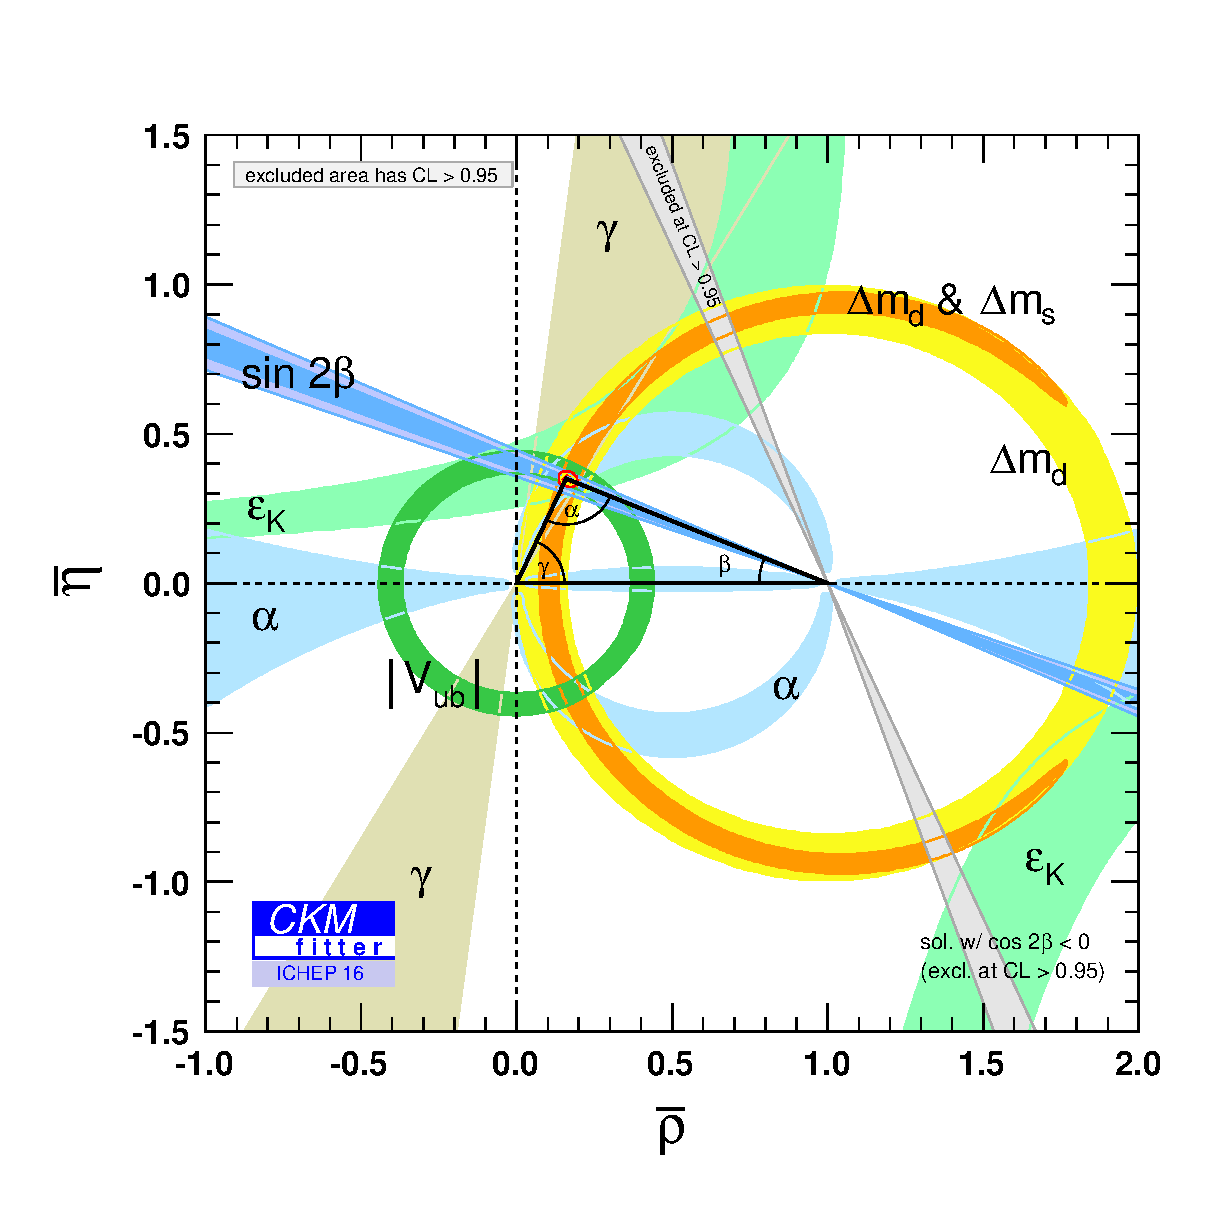
\includegraphics[width=0.7\textwidth]{theory/rhoeta_large_lol.eps}
\vspace*{-1.5cm}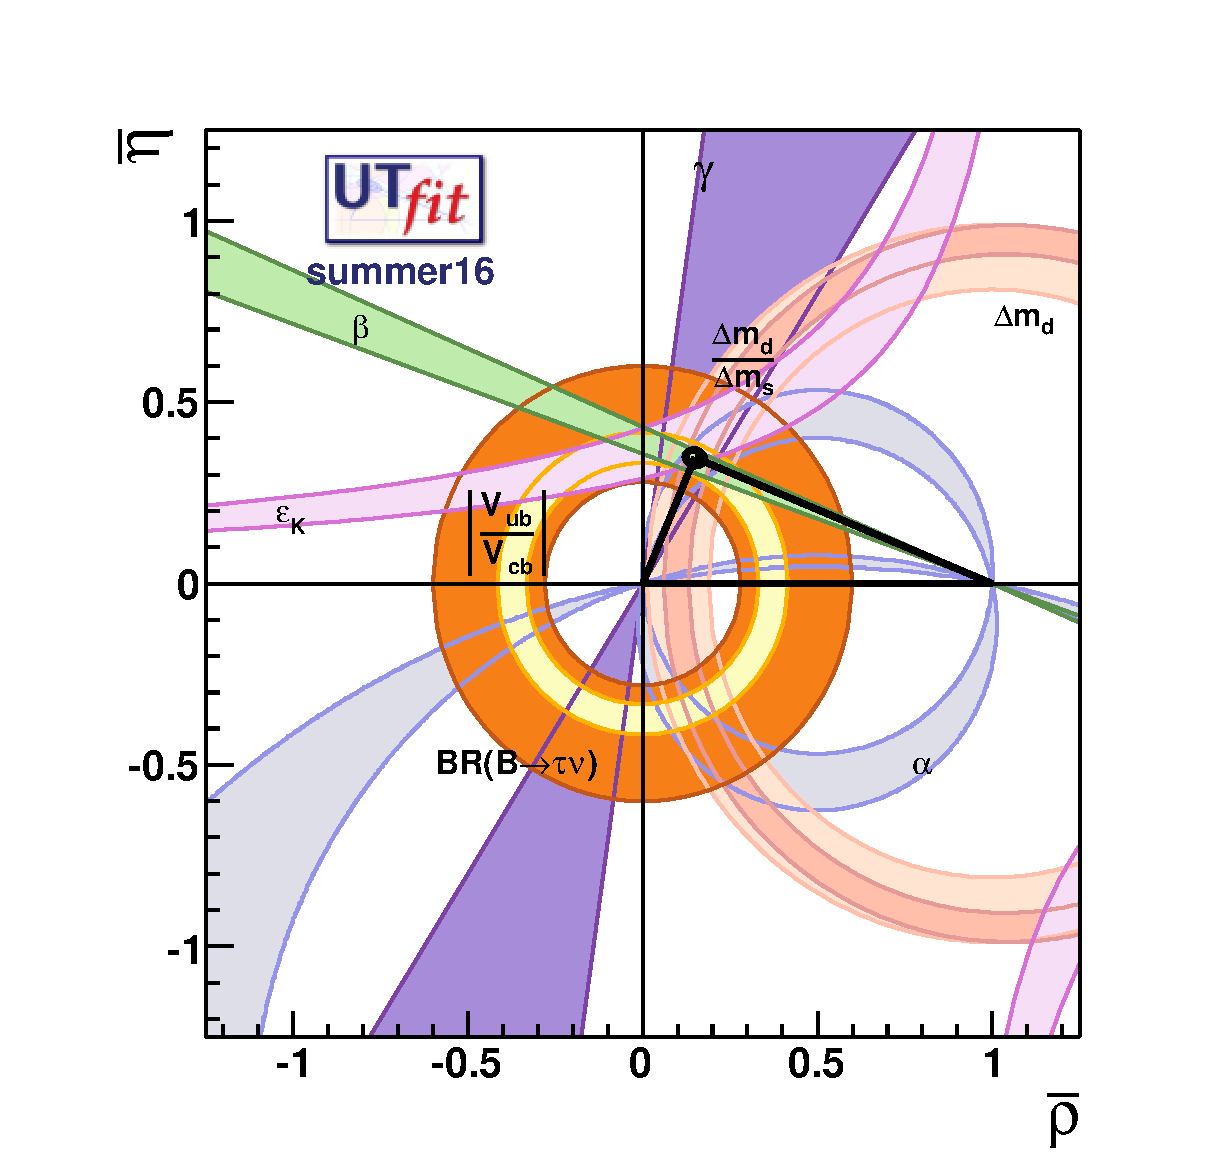
\includegraphics[width=0.65\textwidth]{theory/rhoeta-fullfit-sm.eps}\put(30,130){(a)}
\newline
\hspace*{-1.7cm}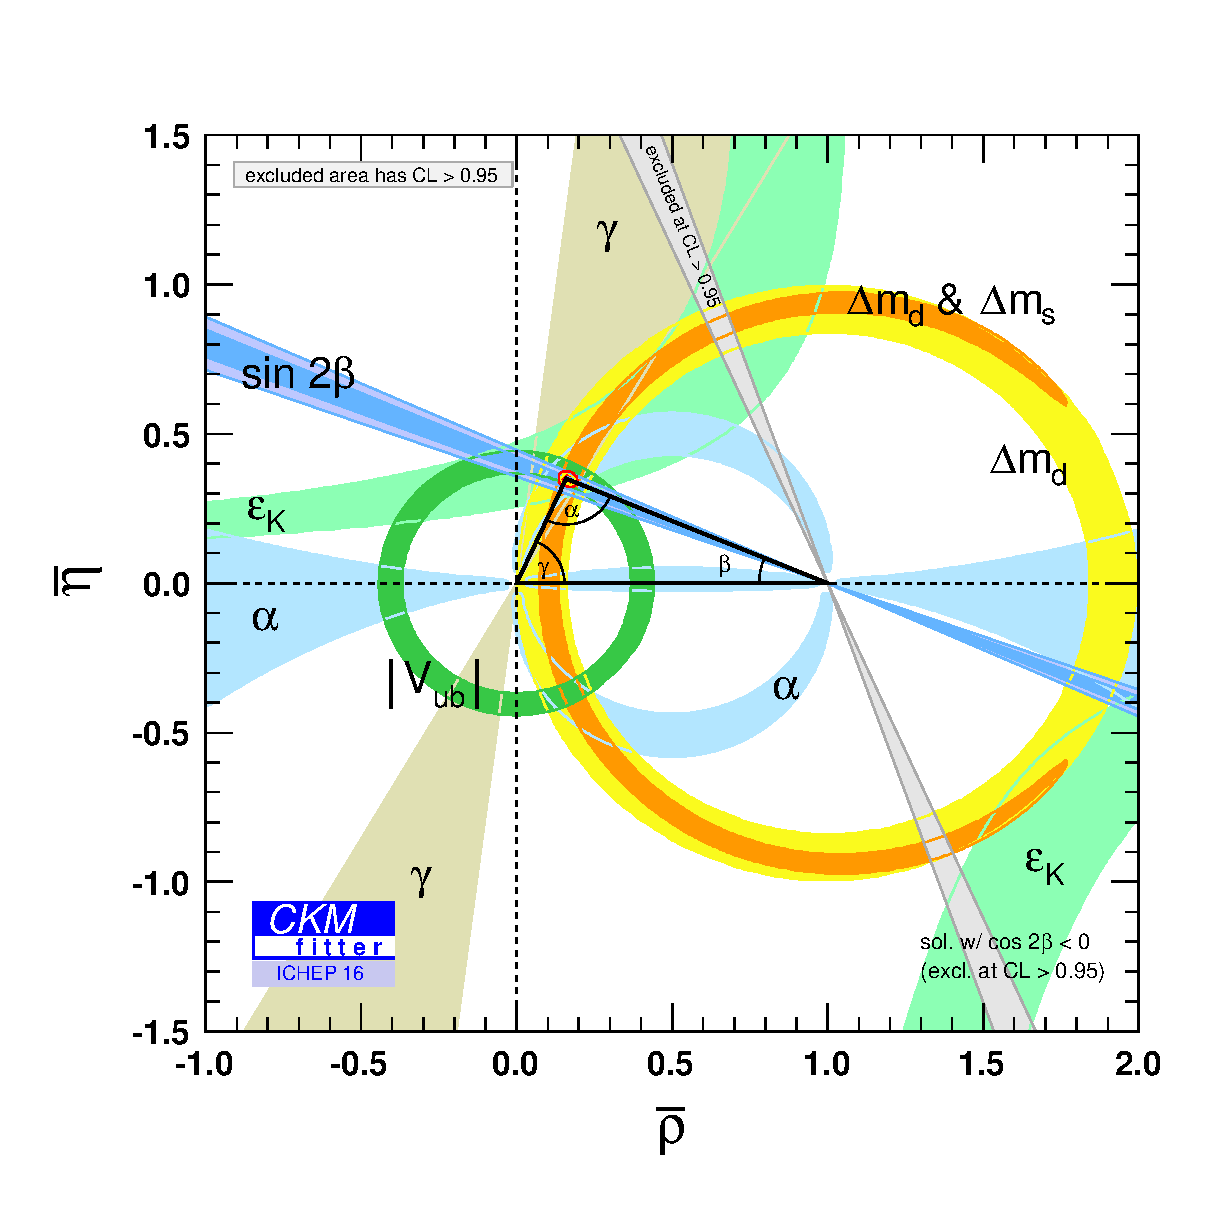
\includegraphics[width=0.65\textwidth]{theory/rhoeta_large_lol.eps}\put(30,130){(b)}
\caption{Different experimental measurements that constrain the \gls{CKM} matrix elements together with the global fit results from two collaborations (a) UTFit and (b) CKMFitter as of summer 2016. This figures are taken from \cite{Bona:2006ah} and \cite{Charles:2004jd}. There is a good agreement for the results between the two different collaborations.}
\label{fig:unifit}
\end{figure}


\section{Fully Leptonic \mb{P^{+}\rightarrow l^{+} \nu_{l}} Decays}
\label{lnudecays}
%This text is based on a summary provided by PDG on Leptonic Decays of Charged Pseudoscalar Mesons.
Purely leptonic decays that proceed via annihilation-type diagrams of pseudoscalar mesons ($P$) are of great interest for flavour physicists because they allow to make:
\begin{itemize}
\item either measurements of the \gls{CKM} matrix elements,
\item or measurements of leptonic decay constants,
\item or measurements of new physics effects.
\end{itemize}
The first two types of measurements are possible because the decay rates of $P^{+}\rightarrow l^{+} \nu_{l}$ decays are sensitive to the product of the appropriate \gls{CKM} matrix element ($V_{q_{1}q_{2}}$ where $q_{1}$ and $q_{2}$ are constituent quarks of the pseudoscalar meson) and decay constant $f_{P}$, related parameter arising from the strong interaction. In more detail, the decay width of a fully leptonic decay of a pseudoscalar meson in the \gls{SM} to the lowest order can expressed as 

\begin{equation}
%\label{eqn:br} 
\Gamma(P^{+} \rightarrow {l^{+}} \nu_{l})=  
	\frac{G_{F}^{2} m^{}_{P^{+}}  m_{l^{+}}^{2}}{8\pi} 
	\left[1 - \frac{m_{l^{+}}^{2}}{m_{P^{+}}^{2}}\right]^{2}  
	f_{P}^{2} |V_{q_{1}q_{2}}|^{2} 
	,
\label{eqn:dw} 
\end{equation}
where
$G_F$ is the Fermi constant,
$m^{}_{P^{+}}$ and $m_{l^{+}}$ are the pseudoscalar meson and lepton masses, respectively. This decay width can be compared to that of $\tau \rightarrow l\nu \bar{\nu}$\cite{Marciano:1988vm}


\begin{equation}
%\label{eqn:br} 
\Gamma(\tau \rightarrow {l} \nu \bar{\nu})=
	\frac{G^{2}_{l\tau} m^{5}_{\tau}}{192\pi^{3}}\left[1-f\big(\frac{m^{2}_{l'}}{{m^{2}_{\tau}}}\big)\right],
\label{eqn:tauonic} 
\end{equation}
where $G_{l\tau}$, is relevant Fermi constant. In this case $ f(x) = 1  8x - 8x^{3} + x^{4} + 12x^{2}log(x)$ represents a correction due to the mass of the lepton
%(finite lepton mass)
in the final state. Corrections arising from the $W$ propagator effects are negligible for this decay and are not considered here and nor are radiative corrections so that only the lowest order contributions are considered. As compared to~\autoref{eqn:dw} the decay width is significantly higher. 

So in order to measure the \gls{CKM} matrix amplitude, knowledge of $f_{P}$ must be inferred. $f_{P}$ can be calculated using lattice \gls{QCD} techniques and together with experimental determination of the decay rates provide a way to determine the amplitude squared of the relevant \gls{CKM} matrix element assuming there is no contribution from new physics. More conventionally, \gls{CKM} magnitudes are determined from semileptonic decays, which is experimentally 
more accesible but entails larger theoretical uncertainty.
%\gls{CKM} magnitudes are determined from semileptonic decays different type of current is given \mybox{this is in pdg i dont understand why is it wrong}. In purely leptonic decays axial-vector flavour-changing currents ($q_{1}\gamma_{\mu}\gamma_{5}q_{2}$) are probed as opposed to vector current ($q_{1}\gamma_{\mu}q_{2}$) in semileptonic case.

Vice versa, assuming unitarity of \gls{CKM} triangle and experimental determination of relevant $V_{q_{1}q_{2}}$ one can obtain experimental determination of the decay constants and compare it with theoretical prediction.

Last, but not least, is of course the measurement of presence of new physics in these decays. Especially appealing is the presence of new particles which would manifest themselves in the decay rates of heavier pseudoscalars ($D_{(s)}$ or $B$). An example of such new particles include charged Higgs bosons, $H^{\pm}$, coming from so-called Type II Higgs-doublet models \cite{Hou:1992sy}\cite{Akeroyd:2003zr}\cite{Dobrescu:2008er} or leptoquarks\cite{Dobrescu:2008er}. In this case, considering $B^{+}\rightarrow l^{+}\nu$ decay, the four-fermion interaction between $W^{\pm}$ and $H^{\pm}$ would modify the \gls{SM} decay width~\autoref{eqn:dw} to
%remember branching fraction is partial width of total width
%total width  h over liftime so lifetime is always missing from equations 
% see https://www2.ph.ed.ac.uk/~vjm/Lectures/ParticlePhysics2010_files/Particle3-2Nov.pdf this

\begin{equation}
\Gamma(B^{+} \rightarrow {l^{+}} \nu_{l})=  
        \frac{G_{F}^{2} m^{}_{B^{+}}  m_{l^{+}}^{2}}{8\pi} 
        \left[1 - \frac{m_{l^{+}}^{2}}{m_{B^{+}}^{2}}\right]^{2}  
	f_{P}^{2} |V_{ub}|^{2} \,\times\, r_H,
%\Gamma(B^+\to \ell^+\nu_\ell)={G_F^2 m_{B} m_l^2 f_{B}^2\over 8\pi}
%|V_{ub}|^2 \left(1-{m_l^2\over m^2_{B}}\right)^2 \,\times\, r_H
\end{equation}
where
\begin{equation}
	r_H=[1-\tan^2\beta(m^{2}_{B^{+}}/m^{2}_{H^{+}})]^2.
\end{equation}
Here $\tan\beta = \frac{v_{2}}{v_{1}}$, where $v_{i}$ are the vacuum expectation values for the Higgs doublets. In order to have an enhancing effect for the rate of the $B^{+}\rightarrow l^{+}\nu$ decay (to have $r_{H}>1$), $\tan\beta/m_{H^{\pm}}> 0.27 \gev^{-1}$. The experimental limit presents already a strong lower bound on the charged Higgs mass $m_{H^{\pm}}>600\gev$\cite{Arbey:2017gmh}. This makes the most of the parameter space in $\tan\beta$ and $m_{H^{\pm}}$ satisfy enhancing condition of $\tan\beta/m_{H^{\pm}}>0.27 \gev^{-1}$.

The ratio of rates between $P\rightarrow\tau\nu$, $P\rightarrow\mu\nu$ and $P\rightarrow e\nu$ decays could also be of an interest. In the ratios the decay constant $f_{P}$ cancels out making such measurements a good tool for lepton universality tests.

As seen in~\autoref{eqn:dw}, a purely leptonic final state going through $P\rightarrow W^{*}\rightarrow l \nu$ is suppressed by $\frac{m^{2}_{l}}{m^{2}_{p}}$, also known as helicity suppression. This suppression occurs as a result of angular momentum conservation. In case of $B^{+}\rightarrow l^{+} \nu$, the $B^{+}$ is a spin-0 particle and hence its decay products should have spin 0 combined, or in other words, be anti-aligned. Neutrinos in the \gls{SM} are always produced left-handed. As the spin of the antilepton and the neutrino should be anti-aligned, the antilepton also needs to be left-handed (to have negative helicity). However, the weak current only couples to right-handed antiparticles. Therefore, the antilepton has to be boosted in order to have different helicity. For massless particles such a helicity flip is not possible making this decay impossible. The lighter the lepton, the larger the velocity and hence higher boost is necessary, making decays to lighter leptons rarer even though they have bigger kinematic phase space available.

%https://www.physicsforums.com/threads/helicity-and-suppression.804600/
Concentraing on the decays $B^{\pm}$ meson, the latest experimental measurements for rates of $B^{+}\rightarrow l \nu$ decays have been performed by $B$ factories, finding evidence for $B^{+}\rightarrow \tau^{+}\nu$ and first sign of $B^{+}\rightarrow \mu^{+}\nu$ as seen in~\autoref{tab:sum}. These results are to be compared with the \gls{SM} predictions $\mathcal{B}(B^{+}\rightarrow \tau^{+}\nu) = (0.82+0.03-0.02)\times10^{-4}$\cite{Charles:2004jd} and $\mathcal{B}(B^{+}\rightarrow \mu^{+}\nu) = (3.80\pm0.31)\times10^{-7}$\cite{Sibidanov:2017vph}, which are obtained by using $|V_{ub}|$ value resulting from other measurements and lattice calculations of $f_{B}$. %Quite substantial statistical as well as systematical errors show the difficulty of this type of measurements. 



\begin{table}[ht]
\begin{center}
\begin{tabular}{ l l l l H c H} \toprule
        Process &Experiment & Tag &${\mathcal{B}}$ & Published & Significance ($\sigma$) & {$|V_{ub}|f_{B^+}$ (MeV)} \hfill\\
\hline\\[-2.5ex]
        $B^{+}\rightarrow \tau^{+}\nu$  &Belle~\cite{Adachi:2012mm}&Hadronic&$(0.72^{+0.27}_{-0.25}\pm0.11)\times10^{-4}$  & 2013 & 3.0 \\
        $B^{+}\rightarrow \tau^{+}\nu$  &Belle~\cite{Kronenbitter:2015kls}&Semileptonic&$(1.25\pm0.28\pm0.27)\times10^{-4}$ & 2015 & 3.8 \\
        $B^{+}\rightarrow \tau^{+}\nu$  &Belle~\cite{Kronenbitter:2015kls}&Average&$(0.91 \pm 0.22)\times10^{-4}$ & 2015 & 4.6 \\\hline\\[-2.5ex]
        $B^{+}\rightarrow \tau^{+}\nu$  &BaBar~\cite{Lees:2012ju} & Hadronic & $(1.83\,^{+0.53}_{-0.49}\pm0.24)\times10^{-4}$ & 2012 & 3.8 \\
        $B^{+}\rightarrow \tau^{+}\nu$  &BaBar~\cite{Aubert:2009wt} & Semileptonic & $(1.7\pm 0.8\pm 0.2)\times10^{-4}$ & 2010 & 2.3\\
        $B^{+}\rightarrow \tau^{+}\nu$  &BaBar~\cite{Lees:2012ju} & Average & $(1.79 \pm 0.48)\times 10^{-4}$ & 2012 & - & $1.01\pm 0.14$  \\ \hline
$B^{+}\rightarrow \mu^{+}\nu$ & Belle~\cite{Sibidanov:2017vph} & Untagged& $(6.46\pm2.22\pm 1.60)\times 10^{-7}$ & 2017 & 2.4 &\\
%        & Our average & &$1.06\pm0.20$&$0.77\pm0.07$ & & \\
\bottomrule
\end{tabular}
\end{center}
\caption{Experimental summary of searches for $B^{+}\rightarrow l^{+}\nu$ that is inspired from \cite{Patrignani:2016xqp}. Tag Hadronic/Semileptonic/Untagged refers to different way data is selected in Belle and BaBar factories.}
\label{tab:sum}
\end{table}




With helicity suppressed rates and very limited signatures in the detector (one charged track for muons and electron, more charged tracks for taus, but also more missing energy depending on the reconstruction channel) searching for such decays is very challenging. In order to make measurements of the same kind (CKM precision measurements, decay constants measurements, new physics searches), fully leptonic decays with photons can be considered.   

\section{Fully Leptonic \mb{B^{+}\rightarrow l^{+} \nu_{l} \gamma} Decays}
\label{lnugamma}
The helicity suppression of $B^{+}\rightarrow l^{+} \nu$ decays can be lifted by considering the decay with an additional photon radiated from the $B^{+}$ meson, at the cost of the electromagnetic suppression with coupling constant $\alpha_{em}$. Consequently, the branching fraction for radiative decays can be comparable or even larger than the corresponding fraction for purely leptonic decays. It has been shown that $R^{\mu}_{B}=\frac{\Gamma(B\rightarrow \mu \nu \gamma)}{\Gamma(B\rightarrow \mu \nu)}\approx(1-20)$ making $\mathcal{B}(B\rightarrow \mu \nu \gamma)\approx(10^{-7}-10^{-6})$ \cite{Burdman:1994ip}.

As compared to photonless decays, the amplitude of the decay will have a contribution from both the axial-vector weak current as well as the vector current.
The differential decay width with $\frac{1}{m_{b}}$ and radiative corrections
at next-to-leading logarithmic order calculated in\cite{Beneke:2011nf} is given by
\begin{equation}
\frac{d\Gamma}{dE_{\gamma}} = \frac{\alpha_{em}G^{2}_{F}|V_{ub}|^{2}}{48 \pi^{2}}m_{B}^{4}(1 - x_{\gamma})x_{\gamma}^{3}[F_A^{2} + F_V^{2}],
\end{equation}
 where $x_{\gamma} = 2E_{\gamma}/m_{B}$, $F_A$ is the axial form factor and $F_V$  is the vector form factor defined as
\begin{equation}
F_{V}(E_{\gamma}) = \frac{Q_{u}m_{B}f_{B}}{2E_{\gamma}\lambda_{B}(\mu)} R(E_{\gamma}, \mu) + [\xi(E_\gamma) +  \frac{Q_{u}m_{B}f_{B}}{(2E_{\gamma})^{2}} + \frac{Q_{b}m_{B}f_{B}}{2E_{\gamma}m_{b}}],
\label{eq:top1}
\end{equation}

\begin{equation}
F_{A}(E_{\gamma}) = \frac{Q_{u}m_{B}f_{B}}{2E_{\gamma}\lambda_{B}(\mu)} R(E_{\gamma}, \mu) + [\xi(E_\gamma) -  \frac{Q_{u}m_{B}f_{B}}{(2E_{\gamma})^{2}} - \frac{Q_{b}m_{B}f_{B}}{2E_{\gamma}m_{b}} + \frac{Q_{l}f_{B}}{E_{\gamma}}].
\label{eq:top2}
\end{equation}
Here $Q_{l},Q_{u},Q_{b}$ are the charges of the lepton, up quark, and
bottom quark, respectively, and $R(E_{\gamma}, \mu)$ is a radiative correction
calculated at the energy scale $\mu$ %that equals one at tree level.
and $m_{b}$ is the mass of the $b$ quark.

The first term in~\autoref{eq:top1} and ~\autoref{eq:top2} represents the leading-power contribution in the heavy-quark expansion. Note that this term
is the same for the vector and axial form factor. The second terms are $\frac{1}{m_{b}}$ power corrections relative to the leading term. Further corrections have been discussed in~\cite{Wang:2016beq}.



Recent measurement of the radiative $B^{+} \rightarrow l^{+} \nu_{l} \gamma$, where $l^{+}$ is either $e^{+}$ or $\mu^{+}$ was performed by Belle using hadronic tagging on their full data sample\cite{Heller:2015vvm}. The search yielded $\mathcal{B}(B^{+}\rightarrow \mu^{+} \nu_\mu \gamma) < 3.4\times 10^{-6}$ and $\mathcal{B}(B^{+}\rightarrow e^{+} \nu_e \gamma) < 6.1\times 10^{-6}$.



\section{Fully Leptonic \mb{B^{+}\rightarrow l^{+} l^{-} l^{+} \nu_{l}} Decays}
\label{mydecay}

In LHCb, the most optimal approach due to the detector capabilities is to measure this kind of decay by converting the photon into a pair of muons, see~\autoref{fig:myfeyn}(a). If the naive expectation of only taking into account photon conversion into two muons is adopted, then the expected branching fraction for this analysis is $\mathcal{B}(B^{+}\rightarrow \mu^{+} \mu^{-} \mu^{+} \nu_{\mu}) \approx 1.0\times 10^{-8}$. However, such estimate is not correct because there are other contributions to the total decay rate as shown in the first theoretical prediction for $\mathcal{B}(B^{+}\rightarrow \mu^{+} \mu^{-} \mu^{+} \nu_{\mu})$ in \cite{Danilina:2018uzr} based on the Vector Meson Dominance (VMD) model. This theoretical prediction yields $\mathcal{B}(B^{+} \rightarrow \mu^{+} \mu^{-} \mu^{+} \nu_{\mu}) \approx 1.3\times 10^{-7}$.% and the rest of this section is a short summary of this publication.

 The VMD model was formulated to describe the interaction between photons and hadrons before \gls{QCD} was formulated. It is an approximative model where the photon is treated to be made of a purely electromagnetic component and a vector meson component. This idea originates in the fact that both photon and vector mesons have the same quantum numbers $J^{PC} = 1^{-\ -}$ and if two particles have the same quantum numbers then they mix. %(the state which commutes with the Hamiltonian is a superposition of all such states). 
% Therefore, there is mixing between photons and vector mesons.

As mentioned previously, there are different contributions to the amplitude of the $\mathcal{B}(B^{+}\rightarrow \mu^{+} \mu^{-} \mu^{+} \nu)$. Using the VMD model, it is not surprising that the biggest contribution arises from the photon emission from the valence $u$-quark of the $B$ meson. In this case, the contribution from the $\rho(770)$ and $\omega(782)$ resonances are included in the calculation. Secondly, the contribution of photon emission from the $b$-quark is studied, effectively creating excited $B^{+}$, $B^{+*}$ intermediate resonance state. Thirdly, the photon can be emitted from the final-state lepton, a process known as Bremsstrahlung. All these different contributions to the decay amplitude are shown in~\autoref{fig:myfeyn}. To obtain the total amplitude, the sum of the matrix elements of the three contributions is calculated in the limit where $m_{l}$ is set to zero.


\begin{figure}[ht]
\centering
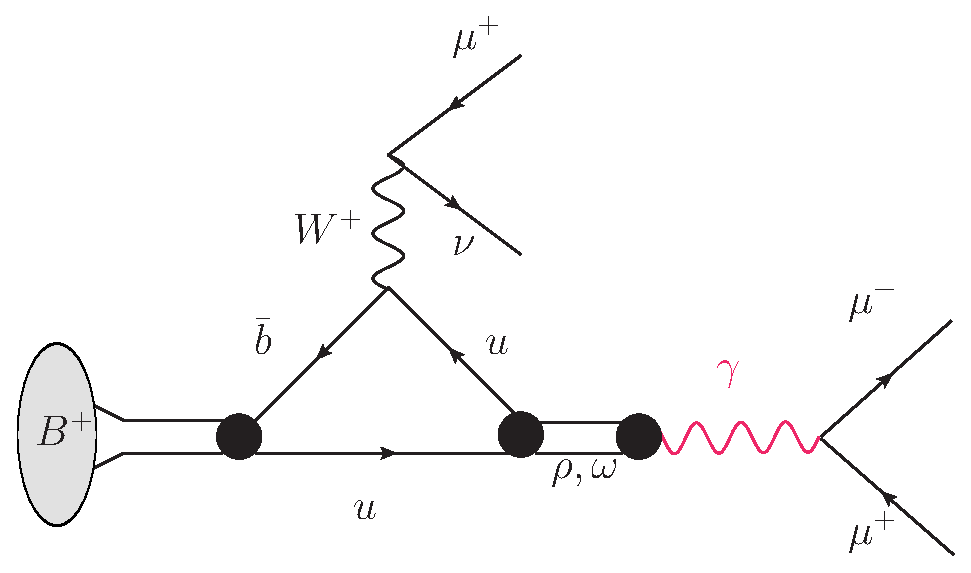
\includegraphics[scale=0.5]{theory/nik_1figure}\put(-30,133){(a)}
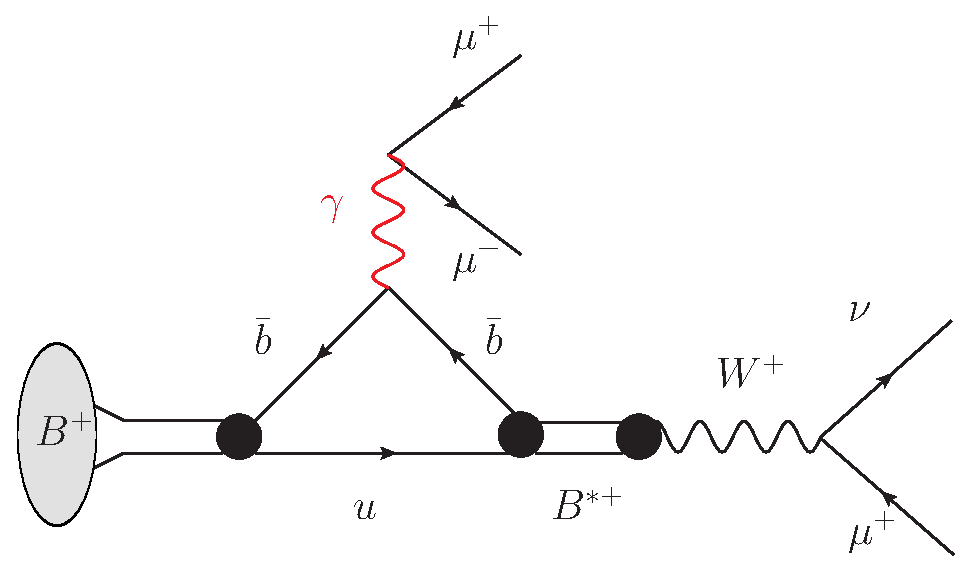
\includegraphics[scale=0.5]{theory/nik_2figure}\put(-30,133){(b)}
\newline
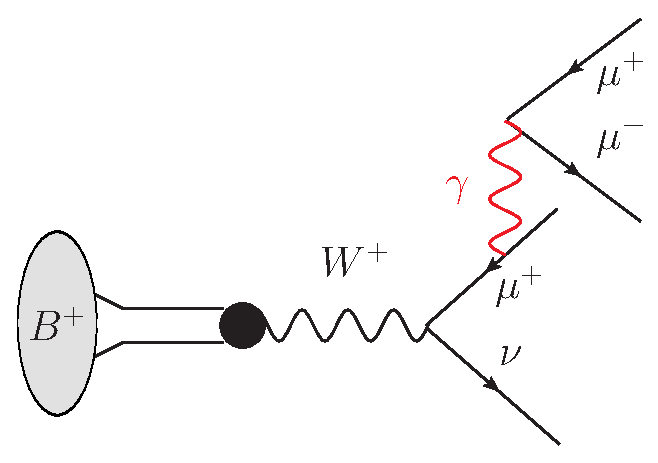
\includegraphics[scale=0.55]{theory/nik_3figure}\put(-30,133){(c)}
\centering
	\caption{Different contributions to the \Bmumumu decay. (a) Initial $u$-quark state radiates off a virtual photon which decays into a pair of muons and the $W^{+}$ decays into a muon and muon neutrino. Most of the contribution to the rate comes from hadronic contribution to the photon. (b) Photon emission from $b$-quark and (c) finally emission from the final state muon.}
\label{fig:myfeyn}
\end{figure}


In this publication the amplitude of $\mathcal{B}(B^{+}\rightarrow \mu^{+} \mu^{-} \mu^{+} \nu)$ is estimated by calculating $\mathcal{B}(B^{+}\rightarrow \mu^{+} \mu^{-} e^{+} \nu)$ amplitude first and then adding a negative interference term that arises due to the identical fermions in the final state doubling the number of possible diagrams. The numerical calculation yields $\mathcal{B}(B^{+}\rightarrow \mu^{+} \mu^{-} e^{+} \nu) \approx 1.3 \times 10^{-7}$ and $\mathcal{B}(B^{+}\rightarrow \mu^{+} \mu^{-} \mu^{+} \nu) \approx 1.3 \times 10^{-7}$. 

\section{The \mb{\Bmumumu} Decay Model}
\label{simulation}
As the search for the \Bmumumu decay is the first of its kind, a simulation that describes this type of decay was not available. There are, however, three types of decay models for \Bmumumu which were adopted and used for different purpose. More detail about their use is covered in~\autoref{SimulationSamples}.

For any decay, it is possible to use a phase space model, \textit{PHSP}, which only takes into account the kinematic constraints of the decay without taking into account any input from theoretical considerations as the matrix element is constant. This is not satisfactory for decays where there are intermediate virtual photons or vector meson resonances.

The following decay model is developed to reflect the expected behaviour of decays shown in~\autoref{fig:myfeyn}. The decay proceeds through a virtual $W$ decaying to $\mu^{+} \nu$ and a virtual photon decaying to a muon pair. This has similar structure to $\B^{+} \rightarrow (K^{*+}) \mu^{+} \mu^{-}$ decay, where the $K^{*+}$ can take the role of the virtual $W$ decay. By using the \textit{BTOSLLBALL} model\cite{Ali:1999mm}, traditionally used for $B^{+} \rightarrow (K^{*+}) l^{+} l^{-}$ decays, but modifying the properties of the $K^{*+}$ to those of virtual $W$ (having mass of 0.1 \gevcc and width 50 \gev), it is possible to obtain a good approximation to the correct features of the decay. This is visible in~\autoref{fig:mcgeneration}, where there is a characteristic photon pole for low $q(\mu^{+},\mu^{-})$, invariant mass of the opposite muon pair, and flat distribution for $K^{*}(\mu^{+}, \nu_{\mu}) $, invariant mass of the muon and neutrino pair. This decay model will be further referred to as \textit{INSP} model. 



%\mybox{Sally: move it to theory and check ulrik's comment} In order to produce simulation with a decay model which is more representative of the spin structure involved, the following strategy is adapted. In this simulation approach, the decay proceeds as follows: \Bpm decays into \Wpm and a pair of opposite sign muons and then \Wp is decayed to $\mu^{+} \nu$. \textit{BTOSLLBALL} model\cite{Ali:1999mm}, traditionally used for $\B \rightarrow (K,K^{*}) l^{+} l^{-}$ decay, with the form factor calculations can be used to simulate $\Bpm \rightarrow \Wpm l^{+} l^{-}$ decay. After that, \Wp is decayed to $\mu^{+} \nu$ using \textit{PHSP}. For semileptonic $b \rightarrow s l^{+} l^{-}$ transitions, there is a characteristic photon pole for low $q(\mu^{+},\mu^{-})$, invariant mass of the opposite muon pair, and flat distribution for $K^{*}(\mu^{+}, \nu_{\mu}) $, invariant mass of the muon and neutrino pair. In order to achieve this, a new pseudo-particle is introduced to EVTGEN with specific properties, $K^{*}(\mu^{+}, \nu_{\mu})$, and the best output can be seen to be for a particle $K^{*}(\mu^{+}, \nu_{\mu})$ with mass to be set to $0.1 \text{GeV/c}^{2}$, and width, corresponding to $\tau= 1.3\times10^{-17}$ nanoseconds as can be seen in~\autoref{fig:mcgeneration}. This procedure was also applied for the charge conjugate case. This model is denoted as \textit{INSP} and is used as default in mass fits and efficiency calculations.

\begin{figure}[h!]
\centering
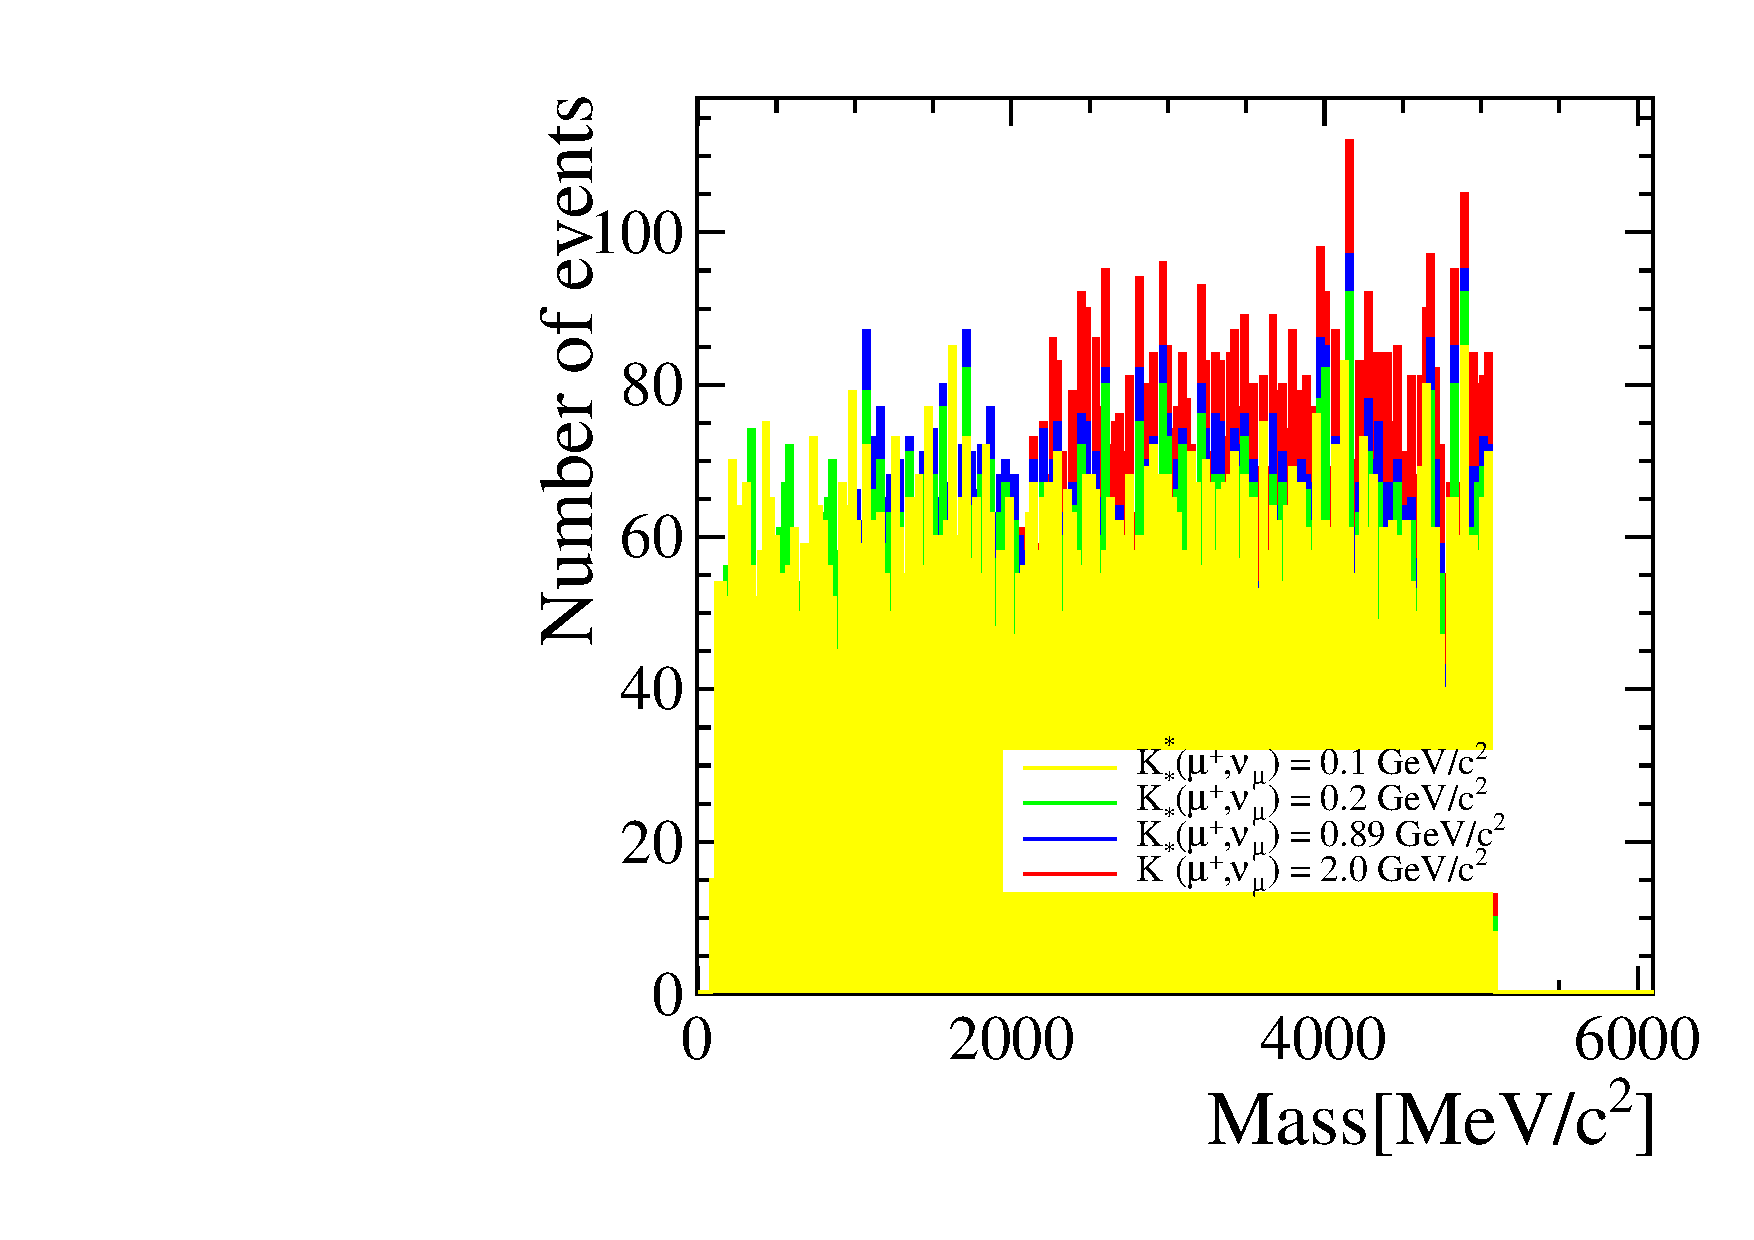
\includegraphics[width=0.5\linewidth]{./sel/reporttry_new}\put(-70,133){(a)}
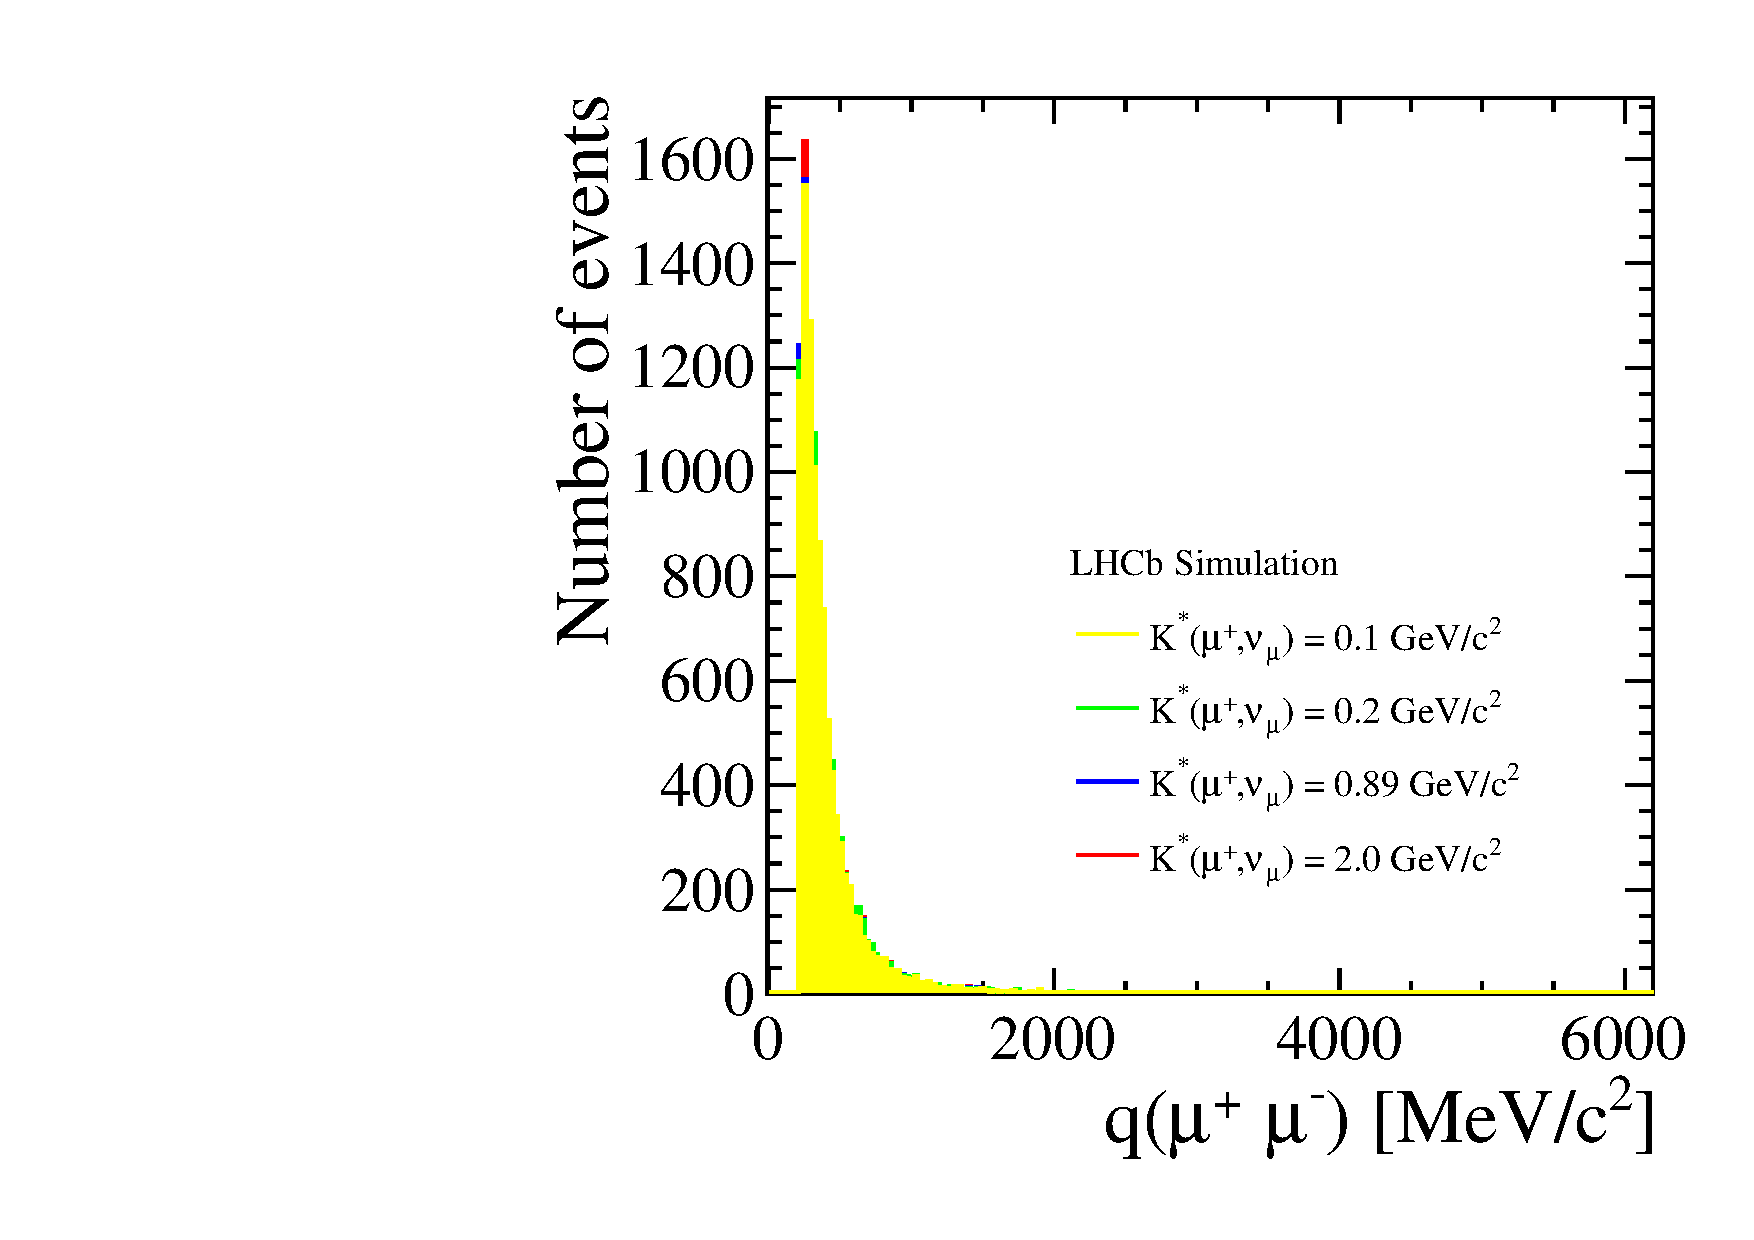
\includegraphics[width=0.5\linewidth]{./sel/reporttrialqpres_new}\put(-50,133){(b)}
\caption{Distributions for signal simulation. (a) $K^{*}(\mu^{+}, \nu_{\mu})$ (b) $q(\mu^{+},\mu^{-})$ distributions under different $K^{*}$ mass hypotheses. The most flat distribution in $K^{*}(\mu^{+}, \nu_{\mu})$ is plotted in yellow.}
\label{fig:mcgeneration}
%\vspace*{-1.0cm}
\end{figure}

Finally, there is a decay model based on calculations from VMD model, which was written by authors of \cite{Danilina:2018uzr}. This model denoted as \textit{NIKI}.

